% Options for packages loaded elsewhere
\PassOptionsToPackage{unicode}{hyperref}
\PassOptionsToPackage{hyphens}{url}
\PassOptionsToPackage{dvipsnames,svgnames,x11names}{xcolor}
%
\documentclass[
  english,
  a4paper,
]{article}
\usepackage{amsmath,amssymb}
\usepackage{lmodern}
\usepackage{iftex}
\ifPDFTeX
  \usepackage[T1]{fontenc}
  \usepackage[utf8]{inputenc}
  \usepackage{textcomp} % provide euro and other symbols
\else % if luatex or xetex
  \usepackage{unicode-math}
  \defaultfontfeatures{Scale=MatchLowercase}
  \defaultfontfeatures[\rmfamily]{Ligatures=TeX,Scale=1}
\fi
% Use upquote if available, for straight quotes in verbatim environments
\IfFileExists{upquote.sty}{\usepackage{upquote}}{}
\IfFileExists{microtype.sty}{% use microtype if available
  \usepackage[]{microtype}
  \UseMicrotypeSet[protrusion]{basicmath} % disable protrusion for tt fonts
}{}
\makeatletter
\@ifundefined{KOMAClassName}{% if non-KOMA class
  \IfFileExists{parskip.sty}{%
    \usepackage{parskip}
  }{% else
    \setlength{\parindent}{0pt}
    \setlength{\parskip}{6pt plus 2pt minus 1pt}}
}{% if KOMA class
  \KOMAoptions{parskip=half}}
\makeatother
\usepackage{xcolor}
\IfFileExists{xurl.sty}{\usepackage{xurl}}{} % add URL line breaks if available
\IfFileExists{bookmark.sty}{\usepackage{bookmark}}{\usepackage{hyperref}}
\hypersetup{
  pdftitle={Estimating the replicability of psychology experiments after an initial failure to replicate},
  pdflang={en},
  colorlinks=true,
  linkcolor={blue},
  filecolor={Maroon},
  citecolor={blue},
  urlcolor={blue},
  pdfcreator={LaTeX via pandoc}}
\urlstyle{same} % disable monospaced font for URLs
\usepackage[margin=25mm]{geometry}
\usepackage{longtable,booktabs,array}
\usepackage{calc} % for calculating minipage widths
% Correct order of tables after \paragraph or \subparagraph
\usepackage{etoolbox}
\makeatletter
\patchcmd\longtable{\par}{\if@noskipsec\mbox{}\fi\par}{}{}
\makeatother
% Allow footnotes in longtable head/foot
\usepackage{footnote} % For some unknown reason, footnotehyper clashes with French
\makesavenoteenv{longtable}
\usepackage{graphicx}
\makeatletter
\def\maxwidth{\ifdim\Gin@nat@width>\linewidth\linewidth\else\Gin@nat@width\fi}
\def\maxheight{\ifdim\Gin@nat@height>\textheight\textheight\else\Gin@nat@height\fi}
\makeatother
% Scale images if necessary, so that they will not overflow the page
% margins by default, and it is still possible to overwrite the defaults
% using explicit options in \includegraphics[width, height, ...]{}
\setkeys{Gin}{width=\maxwidth,height=\maxheight,keepaspectratio}
% Set default figure placement to htbp
\makeatletter
\def\fps@figure{htbp}
\makeatother
\setlength{\emergencystretch}{3em} % prevent overfull lines
\providecommand{\tightlist}{%
  \setlength{\itemsep}{0pt}\setlength{\parskip}{0pt}}
\setcounter{secnumdepth}{5}
% definitions for citeproc citations
\NewDocumentCommand\citeproctext{}{}
\NewDocumentCommand\citeproc{mm}{%
	\begingroup\def\citeproctext{#2}\cite{#1}\endgroup}
\makeatletter
% allow citations to break across lines
\let\@cite@ofmt\@firstofone
% avoid brackets around text for \cite:
\def\@biblabel#1{}
\def\@cite#1#2{{#1\if@tempswa , #2\fi}}
\makeatother
\newlength{\cslhangindent}
\setlength{\cslhangindent}{1.5em}
\newlength{\csllabelwidth}
\setlength{\csllabelwidth}{3em}
\newenvironment{CSLReferences}[2] % #1 hanging-indent, #2 entry-spacing
{\begin{list}{}{%
			\setlength{\itemindent}{0pt}
			\setlength{\leftmargin}{0pt}
			\setlength{\parsep}{0pt}
			% turn on hanging indent if param 1 is 1
			\ifodd #1
			\setlength{\leftmargin}{\cslhangindent}
			\setlength{\itemindent}{-1\cslhangindent}
			\fi
			% set entry spacing
			\setlength{\itemsep}{#2\baselineskip}}}
	{\end{list}}
\usepackage{calc}
\newcommand{\CSLBlock}[1]{\hfill\break\parbox[t]{\linewidth}{\strut\ignorespaces#1\strut}}
\newcommand{\CSLLeftMargin}[1]{\parbox[t]{\csllabelwidth}{\strut#1\strut}}
\newcommand{\CSLRightInline}[1]{\parbox[t]{\linewidth - \csllabelwidth}{\strut#1\strut}}
\newcommand{\CSLIndent}[1]{\hspace{\cslhangindent}#1}

%%%%%%%% START HEADER PARTIAL %%%%%%%%%%%%

% Formatting of tables & knitr::kable and kableExtra functionality
\usepackage{float}
\usepackage{colortbl}
\usepackage{pdflscape}
\usepackage{tabu}
\usepackage{threeparttable}

% Line numbering

% endfloat stuff

% fancyhdr pagestyle

% Environment for keywords
\makeatletter
\newcommand\keywordsname{Keywords}
\newenvironment*{keywords}[1][\keywordsname]{\if@twocolumn \else \small \quotation \fi \begin{center} \textbf{\textit{#1} \\}}{\end{center}\if@twocolumn \else \small \endquotation \fi}
\newenvironment*{keywordsinline}[1][\keywordsname]{\if@twocolumn \else \small \quotation \fi \begin{center} \textbf{\textit{#1}: }}{\end{center}\if@twocolumn \else \small \endquotation \fi}
\makeatother

% Environment for abstract that takes new abstract name
\newenvironment{renameableabstract}[1][\abstractname]{\let\oldabstractname\abstractname \renewcommand{\abstractname}{#1} \begin{abstract}}{\end{abstract} \renewcommand{\abstractname}{\oldabstractname}}

%%%%%%%% END HEADER PARTIAL %%%%%%%%%%%%

\usepackage{tikz}
\usetikzlibrary{positioning,chains}
\usepackage{setspace}\singlespacing
\renewcommand{\textfraction}{0.00}
\renewcommand{\topfraction}{1}
\renewcommand{\bottomfraction}{1}
\renewcommand{\floatpagefraction}{1}
\setcounter{topnumber}{3}
\setcounter{bottomnumber}{3}
\setcounter{totalnumber}{4}
\usepackage{booktabs}
\usepackage{longtable}
\usepackage{array}
\usepackage{multirow}
\usepackage{wrapfig}
\usepackage{float}
\usepackage{colortbl}
\usepackage{pdflscape}
\usepackage{tabu}
\usepackage{threeparttable}
\usepackage{threeparttablex}
\usepackage[normalem]{ulem}
\usepackage{makecell}
\usepackage{xcolor}
\ifXeTeX
  % Load polyglossia as late as possible: uses bidi with RTL langages (e.g. Hebrew, Arabic)
  \usepackage{polyglossia}
  \setmainlanguage[]{}
\else
  \usepackage[main=english]{babel}
% get rid of language-specific shorthands (see #6817):
\let\LanguageShortHands\languageshorthands
\def\languageshorthands#1{}
\fi
\ifLuaTeX
  \usepackage{selnolig}  % disable illegal ligatures
\fi

\title{Estimating the replicability of psychology experiments after an initial failure to replicate}

%%%%%%% START AUTHOR PARTIAL %%%%%%%%%%%%%%%

%%%%% Authors, affiliations and author notes stuff %%%%%

% Macros for creating and referencing stored reference
\makeatletter
\def\MyNewLabel#1#2#3{\expandafter\gdef\csname #1@#2\endcsname{#3}}

\def\MyRef#1#2{\@ifundefined{#1@#2}{???}{\csname #1@#2\endcsname}}

\newcommand*\ifcounter[1]{%
  \ifcsname c@#1\endcsname
    \expandafter\@firstoftwo
  \else
    \expandafter\@secondoftwo
  \fi
}
\makeatother

% Create labels for Addresses if the are given by code
\MyNewLabel{ADDRTXT}{Psych}{Department of Psychology, Stanford University}
\MyNewLabel{ADDRTXT}{GSB}{Graduate School of Business, Stanford University}
\MyNewLabel{ADDRTXT}{Edu}{Graduate School of Education, Stanford University}
\MyNewLabel{ADDRTXT}{Symsys}{Symbolic Systems Program, Stanford University}
\MyNewLabel{ADDRTXT}{Philosophy}{Department of Philosophy, Stanford University}
\MyNewLabel{ADDRTXT}{CS}{Department of Computer Science, Stanford University}

% Create labels for Footnotes if they are given by code
\MyNewLabel{ANOTETXT}{corresp}{Corresponding author. Email: \href{mailto:vboyce@stanford.edu}{\nolinkurl{vboyce@stanford.edu}}}

%%% Special footnotes for addresses and author footnotes
\usepackage{bigfoot}
\DeclareNewFootnote{Addr}[arabic] % Only used for NOT authblk
\DeclareNewFootnote{ANote}[fnsymbol]

%%% Address and author notes as a function of format %%%
 % Use authblk for affiliations %%%%%%%%%%%
\usepackage{authblk}

% Always separate by commas
\renewcommand\Authsep{, }
\renewcommand\Authand{, }
\renewcommand\Authands{, }

% Counter for addresses and footnotes
\newcounter{addrcnt}

% thanks definition that doesnt produce superscript marks
\makeatletter
\newcommand*\createaddrlblbycode[1]{%
  \ifcounter{ADDRLBL@#1}
    {}
    {\refstepcounter{addrcnt}\newcounter{ADDRLBL@#1}\setcounter{ADDRLBL@#1}{\value{addrcnt}}}%
}

\newcommand*\addrlblbycode[1]{\arabic{ADDRLBL@#1}}

\newcommand*\addrbycode[1]{%
  \ifcounter{ADDR@#1}
    {}
    {\newcounter{ADDR@#1}%
     \affil[\addrlblbycode{#1}]{\MyRef{ADDRTXT}{#1}}}%
}

\newcommand*\createanotelblbycode[1]{%
  \ifcounter{ANOTELBL@#1}
    {}
    {\refstepcounter{footnoteANote}\newcounter{ANOTELBL@#1}\setcounter{ANOTELBL@#1}{\value{footnoteANote}}}%
}

\newcommand*\anotelblbycode[1]{\fnsymbol{ANOTELBL@#1}}

\newcommand*\anotebycode[1]{%
  \ifcounter{ANOTE@#1}
    {}
    {\newcounter{ANOTE@#1}%
     \footnotetextANote[\value{ANOTELBL@#1}]{\MyRef{ANOTETXT}{#1}}}%
}
\makeatother


\createaddrlblbycode{Psych}


\createanotelblbycode{corresp}

\author[%
\addrlblbycode{Psych}%
,%
$\anotelblbycode{corresp}$%
]{Veronica Boyce}

\addrbycode{Psych}


\createaddrlblbycode{Psych}



\author[%
\addrlblbycode{Psych}%
]{Ben Prystawski}

\addrbycode{Psych}


\createaddrlblbycode{Psych}



\author[%
\addrlblbycode{Psych}%
]{Adani B. Abutto}

\addrbycode{Psych}


\createaddrlblbycode{Psych}



\author[%
\addrlblbycode{Psych}%
]{Emily M. Chen}

\addrbycode{Psych}


\createaddrlblbycode{GSB}



\author[%
\addrlblbycode{GSB}%
]{Ziwen Chen}

\addrbycode{GSB}


\createaddrlblbycode{Edu}



\author[%
\addrlblbycode{Edu}%
]{Howard Chiu}

\addrbycode{Edu}


\createaddrlblbycode{Psych}



\author[%
\addrlblbycode{Psych}%
]{Irmak Ergin}

\addrbycode{Psych}


\createaddrlblbycode{Psych}



\author[%
\addrlblbycode{Psych}%
]{Anmol Gupta}

\addrbycode{Psych}


\createaddrlblbycode{Symsys}



\author[%
\addrlblbycode{Symsys}%
]{Chuqi Hu}

\addrbycode{Symsys}


\createaddrlblbycode{Philosophy}



\author[%
\addrlblbycode{Philosophy}%
]{Bendix Kemmann}

\addrbycode{Philosophy}


\createaddrlblbycode{Psych}



\author[%
\addrlblbycode{Psych}%
]{Nastasia Klevak}

\addrbycode{Psych}


\createaddrlblbycode{Psych}



\author[%
\addrlblbycode{Psych}%
]{Verity Y. Q. Lua}

\addrbycode{Psych}


\createaddrlblbycode{Edu}



\author[%
\addrlblbycode{Edu}%
]{Mateus M. Mazzaferro}

\addrbycode{Edu}


\createaddrlblbycode{Symsys}



\author[%
\addrlblbycode{Symsys}%
]{Khaing Mon}

\addrbycode{Symsys}


\createaddrlblbycode{Psych}



\author[%
\addrlblbycode{Psych}%
]{Dan Ogunbamowo}

\addrbycode{Psych}


\createaddrlblbycode{Psych}
\createaddrlblbycode{Philosophy}



\author[%
\addrlblbycode{Psych}%
,%
\addrlblbycode{Philosophy}%
]{Alexander Pereira}

\addrbycode{Psych}
\addrbycode{Philosophy}


\createaddrlblbycode{CS}



\author[%
\addrlblbycode{CS}%
]{Jordan Troutman}

\addrbycode{CS}


\createaddrlblbycode{Psych}



\author[%
\addrlblbycode{Psych}%
]{Sarah Tung}

\addrbycode{Psych}


\createaddrlblbycode{Psych}



\author[%
\addrlblbycode{Psych}%
]{Raphael Uricher}

\addrbycode{Psych}


\createaddrlblbycode{Psych}



\author[%
\addrlblbycode{Psych}%
]{Michael C. Frank}

\addrbycode{Psych}


%endif(authblk)

%%%%%%%%% END AUTHOR PARTIAL %%%%%%%%

\date{}

\begin{document}
\maketitle

%%%%%%%%%% START AFTER TITLE PARTIAL %%%%%%%%%%%%%


%%%%%%%%%% END AFTER TITLE PARTIAL %%%%%%%%%%%%%


\begin{otherlanguage}{english}

\begin{abstract}
When a replication fails, scientists have to decide whether to make a second attempt or move on.
Psychology researchers who attempt to replicate studies often face this decision, given the empirical rate of replication success in psychology, which is lower than desired.
Here, we report 17 re-replications of experiments for which an original replication had failed.
In 5/17 of these ``rescue'' projects (29\%), the ``rescue'' study mostly or fully replicated the original results, albeit with a smaller effect size; in the other 12, the second replication was also judged to have failed.
We speculate that successful rescue projects were due to larger sample sizes or methodological changes such as attention checks.
In the absence of obvious weaknesses in a failed replication study's sample or procedure, however, it may be most efficient to stop pursuing an effect after a single failed replication.

\end{abstract}

\end{otherlanguage}

\section{Introduction}\label{introduction}

Imagine you are a graduate student, and you run a replication of a study that you are interested in building upon in your research.
The replication fails.
Perhaps the interaction you hoped for is directionally correct, but the point estimate is small and the confidence interval definitely overlaps 0, with a \(p\)-value of .3.
Or perhaps the interaction is numerically in the wrong direction and the main effects look different.
Whatever the details of the replication failure, you are left with a question: Should you try again and run a re-replication, or should you give up and pick a different study to build upon?

In psychology, large scale replication projects have found that around half of studies successfully replicate.
Across 100 studies with positive results, the reproducibility project in psychology (RP:P) replicated 36\%-47\% depending on the metric for replication success (\citeproc{ref-opensciencecollaboration}{Open Science Collaboration, 2015}).
With large multi-site samples, Many Labs 1 replicated 11/13 effects (84.6\%), Many Labs 2 replicated 14/28 effects (50\%), and Many Labs 3 replicated 3/10 effects (30\%) (\citeproc{ref-ebersole2016}{Ebersole et al., 2016}; \citeproc{ref-klein2014}{Klein et al., 2014}; \citeproc{ref-klein2018}{Klein et al., 2018}).
Camerer et al. (\citeproc{ref-camerer2018}{2018}) examined 21 behavioral social science studies and successfully replicated 12-14 of them (57\%-67\%) depending on the metric used.
Boyce et al. (\citeproc{ref-boyce2023}{2023}) reported an average subjective replication score of 49\% for 176 replications primary in psychology.

Psychology is not the only discipline where many studies do not replicate.
Large scale replication projects in other disciplines have found 39/97 of studies with positive effects (40\%) replicating in cancer biology (\citeproc{ref-errington2021}{Errington et al., 2021}), 11/18 studies (61\%) replicating in economics (\citeproc{ref-camerer2016}{Camerer et al., 2016}), and 31/40 studies (78\%) replicating in experimental philosophy (\citeproc{ref-cova2021}{Cova et al., 2021}).
Across these disciplines, and especially in psychology, large-scale replications indicate a substantial chance of scientists encountering failed replications if they try to replicate published findings.

Replications can fail for many reasons, having to do with the original study or the replication.
Starting with the original study, one potential reason for replication failure is that the original result is fragile in some way.
It could be a statistically unlikely result that was achieved through chance or \(p\)-hacking, or it could be sensitive to the exact conditions and time it was run under (``hidden moderators'').
Another possibility is that the original reported effect size might be inflated due to some combination of heterogeneity, \(p\)-hacking, low power, and publication bias.
A consequence of inflated effect sizes is that replication studies might select a sample size with appropriate statistical power for the reported effect size and then have too small a sample to reliably detect the (true) smaller effect.
Replication studies might also end up underpowered due to unexpected attrition or noise in the replication sample.

Some other reasons for replication failure are primarily due to the replication study.
A replication could observe different results from the original due to methodological differences.
These differences in design could be intentional adaptations, unavoidable changes from lack of access to the original instructions or materials, or changes that were not expected to be critical.
A difference in the details of recruitment (e.g., online versus in-person) might mean that particular details of a study implementation would no longer be appropriate, or the data quality controls and attention checks might be inadequate.
If there are differences in time, place, or subject population between the two studies, corresponding changes to the materials, instructions, or procedure could be needed to provide an adaptation of the experimental paradigm to the new context.
Such adaptation creates yet more challenges in interpretation: too many changes could cause differing results, but so could not enough changes.
In sum, when replications fail, we generally do not know why they failed, although we may speculate.

For the goals of large-scale replication projects, it does not matter why any particular study failed to replicate, because the aim is to estimate the proportion of replication effects in a literature.
In contrast, however, when individual scientists attempt to replicate an effect with the goal of building on it, they do care about why an individual replication failed.
In an uncertain literature, scientists might not want to commit resources to studying extensions of an effect without first checking that they can measure that effect themselves.
For those individual scientists, it is much more important whether the replication failure is due to a fixable issue with the replication or an intrinsic feature of the original result.

Re-replication can serve as a way to test explanations for replication failure.
While it is possible to speculate after the fact about potential causes of a single replication failure, in most circumstances these causes are hard to discern (absent clear evidence of errors).
In contrast, a second replication provides a chance to test explanations by making modifications -- as well as giving another chance for researchers to measure an effect of interest.
But what are the chances that a re-replication succeeds?

Relatively few studies have estimated re-replication success.
One estimate comes from Ebersole et al. (\citeproc{ref-ebersole2020}{2020}).
After the original RP:P study reported of a replication rate around 40\% (\citeproc{ref-opensciencecollaboration}{Open Science Collaboration, 2015}), Gilbert et al. (\citeproc{ref-gilbert2016}{2016}) raised concerns that methodological differences might explain the low replication rate.
In 11 of the RP:P studies, the original authors had raised concerns about protocol fidelity prior to data collection.
Of these 11 with concerns, 10 failed to obtain significant results in the RP:P replication.
Thus, Ebersole et al. (\citeproc{ref-ebersole2020}{2020}) re-replicated 10 of these 11 in larger samples, using both the RP:P protocol and a new protocol revised under advice of the original authors or other experts.
This study thus tested whether larger sample sizes and/or ``better'' methodologies would ``rescue'' the failed RP:P replications.
The result was that 2 of the 10 revised protocols found a significant result (but not the 1/11 that originally was successful).
Even when a significant effect was recovered, the effect size was much diminished (\citeproc{ref-ebersole2020}{Ebersole et al., 2020}).
The re-replication success rate was thus 2/9 (22\%) for studies with non-significant first replications, under favorable, high-resource circumstances.

While Ebersole et al. (\citeproc{ref-ebersole2020}{2020}) looked at re-replication success rate in a high resource setting with access to large, multi-site samples and expert input, most early career scientists do not have those kinds of resources to devote to re-replication attempts.
On the other hand, early career researchers may also be prone to a different distribution of causes of initial replication failure.
Thus, it is an open question what the re-replication rate is for failed replications by early career researchers.
Further, estimating this rate could inform researchers' decisions on what to do next after failed replications.

Here, we investigate re-replication in the context of graduate student replication class projects.
Students in a graduate-level class on experimental methods in psychology were given the option to ``rescue'' an experiment that a student in a prior year had previously failed to replicate as their class project (first replications reported in \citeproc{ref-boyce2023}{Boyce et al., 2023}).
The focus of the class was best practices in experimental design; thus, students looked at both the original paper and the failed replication to examine potential issues in the replication that they could fix in their rescue project.
In the present paper, we report the results of 17 re-replication rescue projects.
We find that a minority of projects (5/17, 29\%) successfully recovered the original effect.

\section{Methods}\label{methods}

PSYCH 251 is a graduate-level experimental methods class taught by MCF.
In previous years, students have conducted replication projects (\citeproc{ref-boyce2023}{Boyce et al., 2023}; \citeproc{ref-hawkins2018}{Hawkins et al., 2018}).
In Fall 2023, students were offered the option to complete a ``rescue'' project where they re-replicated one of the unsuccessful replications from a previous year.
Students could also opt to do a normal replication instead.
If they opted for a rescue, they were given the option to participate in a collaborative meta-science project and earn authorship on the current paper based on 1) completing a rescue project, 2) reviewing another student's rescue project for reproducibility, and 3) reviewing and approving the final manuscript.
We report on the result of 17 rescue projects that opted to be part of the paper and completed data collection.

A spreadsheet of projects, individual project write-ups (both first replications and rescues), individual project data and analyses for rescue projects, and the analytic code for this paper are all available at \url{https://osf.io/cyk5w/}.

Our analysis plan was pre-registered after students had selected projects, but before final data collection on the projects.
Each project was also individually pre-registered by the student conducting it.
The overall analysis is pre-registered at \url{https://osf.io/5qz7v}, individual pre-registrations are linked from \url{https://osf.io/vkbfw}.
We note one deviation from our pre-registration here: we pre-registered visual comparisons between original, first replication, and rescue projects using prediction intervals.
Prediction intervals depend on both the original effect size and variance and the variance of the comparison (replication or rescue) study (\citeproc{ref-patil2016}{Patil et al., 2016}).
Thus we cannot show a single prediction interval for the original study, but would have to show a prediction interval between each pair of studies.
We thought this analysis would not offer additional clarity and hence we did not perform it.

\subsection{Sample}\label{sample}

The experiments that were re-replicated were chosen from studies that failed to replicate in Boyce et al. (\citeproc{ref-boyce2023}{2023}).
We created an initial list of 49 rescue-eligible studies that 1) had received a subjective replication success score of 0, .25, or .5 (on a 0--1 scale) in Boyce et al. (\citeproc{ref-boyce2023}{2023}), 2) had a Github repository available (Github repositories were used in class starting in academic year 2015-2016), and 3) where the original experiment had 200 or fewer participants (to ensure we could afford to match or increase the sample size based on the class budget).
We then contacted the replication project authors for permission to share their report and repository with a new student and include it as a supplement on a resulting paper.
This left 27 options for the students to choose from.
20 students chose to do rescue projects, and 3 students did not finish their project or did not indicate interest in being part of this paper, leaving a final sample of 17 rescue projects.

\subsection{Procedure}\label{procedure}

Students conducted their rescue projects over the course of the 10-week class.
Once they had chosen a project we gave them access to the original replicators' write-up and repository, which often included the data, experiment code, and analytic code.
In many cases, students were also given the contact information of the original replicator (a few original replicators opted not to be contacted by students).

Students were required to think of reasons the first replication might not have worked, and address them if they could.
A list of possible reasons and solutions was given to students (\url{https://osf.io/dfwk2}).
In general, we encouraged students to add manipulation checks as appropriate, and to adapt their materials to online studies, which may benefit from attention checks and/or shorter duration.
For instance, the rescue of Paxton et al. (\citeproc{ref-paxton2012}{2012}) switched from using the Cognitive Reflection Test (CRT) which many online participants are over-familiar with to using the newer CRT-2 which is less overused but attempts to measure the same construct (\citeproc{ref-thomson2016}{Thomson \& Oppenheimer, 2016}).
The rescue of Jara-Ettinger et al. (\citeproc{ref-jara-ettinger2022}{2022}) discovered that the replication had accidentally used an illustrated version of the stimuli rather than the photographic stimuli used in the original and used the photographic stimuli instead.
Tarampi et al. (\citeproc{ref-tarampi2016}{2016}) had participants do a timed navigation task where they wrote L or R to indicate which way to turn at each intersection on a paper map.
The replication ported this experiment online and had participants click a drop down menu to select left or right for each turn.
The rescue removed the unwieldy drop down menus and opted to have participants press keys on the keyboard to indicate the direction of a turn, which seemed like a more natural interface.
Once experimental designs and analytic plans were approved by class TAs (VB and BP), students pre-registered and ran their samples.

With one exception, samples were collected on Prolific (the rescue of \citeproc{ref-yeshurun2003}{Yeshurun \& Levy, 2003} ran in-person on the Stanford student subject pool).
We tried to power studies adequately (with a target of 2.5x original following \citeproc{ref-simonsohn2015}{Simonsohn, 2015}), but due to cost constraints, not all studies were powered at this level.
The rescues had on average 1.48 times the original sample post-exclusion (median: 1.07, IQR: 0.94 - 2.4, minimum: 0.48, maximum: 2.96, see Table \ref{tab:tab-size} for all sample sizes).
Across the 16 Prolific studies, we spent \$5471, for an average of \$342 per project.

\subsection{Coding of results}\label{coding-of-results}

We followed Boyce et al. (\citeproc{ref-boyce2023}{2023}) in the properties of the studies we measured and how we quantified replication success.
Each project was rated on the basis of subjective replication success (on a 0--1 scale) by both MCF and one of VB and BP.
We thought about replication in terms of general match in key study results (direction, magnitude, and significance), rather than focusing on any singular numeric result or significance cut-off.
Interrater reliability was 0.9; disagreements were minor (at no point greater than .25) and were resolved through discussion.

As a complement to the subjective rating of overall success, we statistically compared one key measure of interest for each study, following Boyce et al. (\citeproc{ref-boyce2023}{2023}).
In order to statistically compare the key measures, we needed effect sizes reported in the same way for each original study, first replication, and rescue.
When effects were not reported in consistent ways across original and replications, we recalculated effects from raw data when necessary to obtain comparable values.

We measured statistical consistency using \(p\)-original, the \(p\)-value on the null hypothesis that one study's population effect comes from the same distribution of population effects as another study or studies (\citeproc{ref-mathurNewStatisticalMetrics2020a}{Mathur \& VanderWeele, 2020}) If we assume no heterogeneity between studies, then this is the same as asking how consistent one study's estimate of the population-level effect is with another study's estimate of the population-level effect.
However, meta-analyses of closely related studies, such as those from different sites of multi-site replications, indicate that there is often heterogeneity between studies.
\(p\)-original allows for such heterogeneity, as governed by a parameter \(\tau\).
We cannot accurately estimate the level of heterogeneity for an effect meta-analytically as we have only a small number of replications per study.
Instead, we imputed a heterogeneity value of \(\tau=.21\) SMD, which is the average level of heterogeneity found by Olsson-Collentine et al. (\citeproc{ref-olsson-collentine2020}{2020}) in prior multi-site replications in psychology.

We recorded the same set of potential correlates that were used in Boyce et al. (\citeproc{ref-boyce2023}{2023}) for original, first replication, and rescue (these were already rated for original and first replication).
These potential correlates included the subfield of the study (cognitive, social, or other psychology), its publication year, experimental design features including whether it was a within- or between-subject design, whether each condition was instantiated with one vignette or multiple, how many items each participant saw, and whether there were open materials and open data.

For the original study and each replication, we recorded the number of participants post-exclusions.
For studies where some extra conditions were dropped in some replications, we counted only the participants in the key conditions all replications had for comparability.
For instance, if an original study compared between two critical conditions but also had a baseline control, we did not count the participants in the baseline condition if a replication did not include this condition.
We also recorded whether each study was conducted online using a crowd-sourced platform or not.

\section{Results}\label{results}

We first discuss the overall rate of replication in the rescue projects, followed by looking at the relative effect sizes of the rescues and correlates of rescue success.
In the last subsection we describe several interesting case studies.

\subsection{Overall replication rate}\label{overall-replication-rate}

Our primary question of interest was how many of the 17 rescue projects succeeded at replicating the results in the original study.
Across the 17 rescue projects, 5 mostly or fully replicated the original results according to the subjective replication ratings.
12 got a rating of 0, 2 got a rating of .75, and 3 got a rating of 1.
Thus, a first pass answer to the question ``how often can a failed replication be salvaged?'' is 29\% (bootstrapped 95\% CI: 12\% - 53\%) of the time.

In the original replication sample from Boyce et al. (\citeproc{ref-boyce2023}{2023}), 76 out of 176 replications (43\%) mostly or fully replicated (i.e.~received a subjective replication score of .75 or 1).
Note that Boyce et al. (\citeproc{ref-boyce2023}{2023}) report the average replication score as a percent success (49\%), but given that we considered studies with a subjective score of .5 as eligible to be rescued, we recomputed the success rate where scores of 0, .25, and .5 are considered failures and .75 and 1 successes.
If the re-replication rate in our sample is representative of the re-replication rate for the initially non-replicating studies, then the combined chance of mostly or fully replicating in a first replication or one follow-up replication is 60\%.

\subsection{Effect size comparison}\label{effect-size-comparison}

\begin{figure}
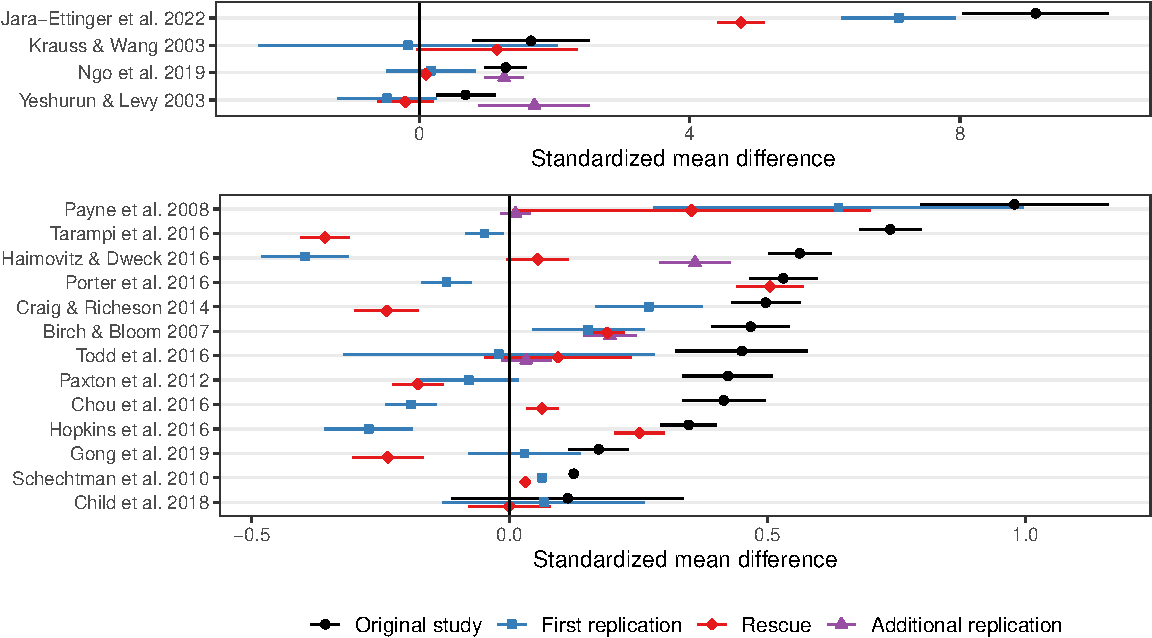
\includegraphics[width=1\linewidth]{manuscript_files/figure-latex/smd-1} \caption{Standardized effect sizes of original studies, first replications, rescues, and additional replications if available. Due to the large effect size of a couple studies, large effect studies are shown in a separate panel. In a few cases, the first replication's key effect was in the same direction as the original with a 95\% CI that did not overlap 0; however, in these cases the larger pattern of results was not consistent between original and first replication.  }\label{fig:smd}
\end{figure}

As a complement to subjective replication ratings, we also statistically compared the effect sizes of the rescue, first replication, and original study on one preregistered key measure per study (again following \citeproc{ref-boyce2023}{Boyce et al., 2023}).
Though we did not conduct a systematic review of the literature to identify all possible replications, we also consider the effect sizes obtained in additional replications when we were aware of them (either from other class projects, or external replications in the literature).

We standardized all effect sizes into standardized mean difference (SMD) units.
One potential issue with comparisons using SMD is that noisier measures will have smaller standardized effect sizes even if the effect on the original scale is the same.
In general, the replication and rescue effect sizes were smaller than the original effect sizes, and in a few cases the effects were in the opposite direction (Figure \ref{fig:smd}).

\begin{table}

\caption{\label{tab:tab-porig}$P$-original values between different sets of experiments. The primary analysis is between the original result and the meta-analytic aggregation of all replications. All $p$-original values assume an imputed heterogeneity value of $\tau$=.21.}
\centering
\begin{tabular}[t]{lrrrrr}
\toprule
\multicolumn{1}{c}{ } & \multicolumn{5}{c}{p-original comparing between} \\
\cmidrule(l{3pt}r{3pt}){2-6}
\multicolumn{1}{c}{ } & \multicolumn{4}{c}{Original and} & \multicolumn{1}{c}{Rescue and} \\
\cmidrule(l{3pt}r{3pt}){2-5} \cmidrule(l{3pt}r{3pt}){6-6}
Paper & All reps & 1st Rep and Rescue & Rescue & Non-rescue & Other reps\\
\midrule
Birch \& Bloom 2007 & 0.192 & 0.189 & 0.194 & 0.191 & 0.989\\
Child et al. 2018 & 0.669 & 0.669 & 0.641 & 0.858 & 0.778\\
Chou et al. 2016 & 0.055 & 0.055 & 0.101 & 0.005 & 0.231\\
Craig \& Richeson 2014 & 0.145 & 0.145 & 0.001 & 0.302 & 0.020\\
Gong et al. 2019 & 0.262 & 0.262 & 0.057 & 0.511 & 0.228\\
Haimovitz \& Dweck 2016 & 0.068 & 0.018 & 0.018 & 0.180 & 0.867\\
Hopkins et al. 2016 & 0.290 & 0.290 & 0.654 & 0.004 & 0.015\\
Jara-Ettinger et al. 2022 & 0.014 & 0.014 & 0.000 & 0.006 & 0.000\\
Krauss \& Wang 2003 & 0.271 & 0.271 & 0.519 & 0.139 & 0.311\\
Ngo et al. 2019 & 0.106 & 0.000 & 0.000 & 0.385 & 0.257\\
Paxton et al. 2012 & 0.011 & 0.011 & 0.005 & 0.023 & 0.649\\
Payne et al. 2008 & 0.023 & 0.071 & 0.031 & 0.079 & 0.895\\
Porter et al. 2016 & 0.370 & 0.370 & 0.905 & 0.002 & 0.003\\
Schechtman et al. 2010 & 0.712 & 0.712 & 0.654 & 0.770 & 0.877\\
Tarampi et al. 2016 & 0.000 & 0.000 & 0.000 & 0.000 & 0.145\\
Todd et al. 2016 & 0.062 & 0.100 & 0.124 & 0.058 & 0.778\\
Yeshurun \& Levy 2003 & 0.614 & 0.007 & 0.017 & 0.943 & 0.474\\
\bottomrule
\end{tabular}
\end{table}

Scientists' intuitions about whether a replication is successful and whether an effect provides support for a hypothesis (including heuristic cutoffs like p\textless.05) do not always align with measures of statistical consistency (\citeproc{ref-patil2016}{Patil et al., 2016}).
For instance, two studies may both find that condition 1 results in a significantly higher outcome measure than condition 2, but the effect magnitudes may be sufficiently different that they are statistically unlikely to have come from the same population.
On the other hand, one study may find a statistically significant, but imprecisely estimated effect in a small sample, and a second study may find a near-zero (null) effect, but the effect estimates from the two studies may be statistically compatible, despite one supporting a hypothesized difference and the other not.

As our primary comparison, we compare the effect size of the original study to the meta-analytic effect of the totality of the replications (first replication, rescue, and additional if found).
The value of \(p\)-original represents how likely an effect size equal to or more extreme than the original effect size is to occur if it comes from a distribution of population effect sizes defined by the mean and standard error of the replications (combined meta-analytically) with a between-population standard deviation of \(\tau=.21\) (imputed from \citeproc{ref-olsson-collentine2020}{Olsson-Collentine et al., 2020}).
That is, \(p\)-original is a measure of the statistical consistency of the original result with the totality of the replications, assuming a given level of heterogeneity of effects between studies.
Smaller \(p\)-original values indicate more inconsistency.

The median value of \(p\)-original between an original study and its replications was 0.15 {[}IQR: 0.05 - 0.29{]}.
24\% of the \(p\)-original values were less than .05, indicating by conventional thresholds a rejection of the null hypothesis that the original comes from the same distribution of population effects as the replications.
Individual \(p\)-original values for each study are shown in Table \ref{tab:tab-porig}.

As secondary measures, we calculated the \(p\)-original values between a) the original and just the first replication and rescue (i.e.~excluding additional replications), b) the original and the rescue, c) the original and non-rescue replications, and d) the rescue and other replications.
For a) the original versus the first replication and the rescue, the median value of \(p\)-original was 0.1 {[}IQR: 0.01 - 0.27{]}, and 35\% of the \(p\)-original values were less than .05.
For b) the original versus the rescue, the median value of \(p\)-original was 0.06 {[}IQR: 0.01 - 0.52{]}, and 47\% of the \(p\)-original values were less than .05.
For c) the original versus all the non-rescue replications, the median value of \(p\)-original was 0.14 {[}IQR: 0.01 - 0.38{]}, and 35\% of the \(p\)-original values were less than .05.
For d) the rescue versus the other replications, the median value of \(p\)-original was 0.31 {[}IQR: 0.14 - 0.78{]}, and 24\% of the \(p\)-original values were less than .05.

Overall, allowing for a heterogeneity level of \(\tau\)=.21 SMD, a number of original effects are not statistically consistent with rescue and replication effects.
The pattern of inconsistency does not align with which studies were rated as having replicated.
In all cases, the point estimate of the re-replication is smaller than, or in the opposite direction of, the original effect on the key measure of interest.

\subsection{Correlates of rescue success}\label{correlates-of-rescue-success}

\begin{table}

\caption{\label{tab:cor-table}Correlations between an individual predictor and the subjective replication score of the rescue project. The first set of predictors were pre-registered based on the correlates used in Boyce et al. (2023). Original authors at Stanford refers to at the time of the first replication as this may mean the first replication was not independent. For details about how the predictors were coded, see the Methods section of Boyce et al. (2023). The last three predictors were added post-hoc.}
\centering
\begin{tabular}[t]{rcc}
\toprule
Predictors & r & p\\
\midrule
Social & 0.133 & 0.612\\
Other psych & -0.295 & 0.250\\
Within subjects & 0.210 & 0.418\\
Single vignette & -0.030 & 0.910\\
Switch to online & 0.175 & 0.501\\
Open data & 0.231 & 0.373\\
Open materials & 0.471 & 0.057\\
Original authors at Stanford & -0.233 & 0.369\\
Log number of trials & 0.005 & 0.985\\
Log original sample size & 0.027 & 0.919\\
Log rescue/original sample size & 0.024 & 0.927\\
\midrule\\
Log replication sample size & -0.258 & 0.317\\
Log replication/original sample size & -0.487 & 0.048\\
Log rescue/replication sample size & 0.490 & 0.046\\
\bottomrule
\end{tabular}
\end{table}

Are there signals in the features of original or replication studies that predict whether a re-replication will succeed?
To address this question, we report correlations between the set of predictor variables used in Boyce et al. (\citeproc{ref-boyce2023}{2023}) and the subjective replication scores of the rescues.
We also added some (non-preregistered) predictors related to the sample size of the first replication, after seeing the successful re-replications of Ngo et al. (\citeproc{ref-ngo2019}{2019}) and Krauss \& Wang (\citeproc{ref-krauss2003}{2003}), both of which had small replication samples and larger rescue samples.

All of the correlations are presented in Table \ref{tab:cor-table}.
The number of rescues is small, and many of these predictors are correlated, so we caution against over interpretation.

The strongest correlates of rescue success were open materials, a small sample size on the first replication, a small sample size on the first replication relative to the original sample size, and a large rescue sample size relative to the first replication.
None of the pre-registered correlates meet the conventional significance threshold; the two correlates based on ratios that reflect a relatively smaller replication sample size are marginally significant.

Small replication samples relative to original and rescue could be due to both a) powering a replication according to a reported large effect size or b) difficulties with recruitment or high exclusion rates leading to a smaller than intended sample.
Since relative sizes of the studies may play a role in replication success and how probative replications are, we show the sample sizes in Table \ref{tab:tab-size}.

An additional factor that influences the interpretation of a replication is how close the replication's methods were to the original.
In the rescue projects, we aimed to have methods be as close as was feasible or appropriate.
However, rescue projects varied in how close the re-replications actually were, often due to limitations in the availability of original stimuli and original instructions, in addition to the use of primarily online subject pools.
Table \ref{tab:tab-size} shows the closeness of each first replication and rescue according to the classification scheme from LeBel et al. (\citeproc{ref-lebel2018}{2018}).

\begin{table}

\caption{\label{tab:tab-size}Comparison of sample size for original, replication, and rescue samples and measures of closeness for replication and rescue samples.}
\centering
\begin{tabular}[t]{lllllll}
\toprule
\multicolumn{1}{c}{Paper} & \multicolumn{1}{c}{Score} & \multicolumn{3}{c}{N} & \multicolumn{2}{c}{closeness} \\
\cmidrule(l{3pt}r{3pt}){1-1} \cmidrule(l{3pt}r{3pt}){2-2} \cmidrule(l{3pt}r{3pt}){3-5} \cmidrule(l{3pt}r{3pt}){6-7}
 &  & Original & Replication & Rescue & Replication & Rescue\\
\midrule
Krauss \& Wang 2003 & 1.00 & 101 & 19 & 75 & close & very close\\
Ngo et al. 2019 & 1.00 & 31 & 12 & 77 & very close & very close\\
Todd et al. 2016 & 1.00 & 63 & 26 & 55 & very close & very close\\
Jara-Ettinger et al. 2022 & 0.75 & 144 & 147 & 426 & exact & exact\\
Porter et al. 2016 & 0.75 & 145 & 168 & 136 & close & close\\
Birch \& Bloom 2007 & 0.00 & 103 & 73 & 247 & very close & very close\\
Child et al. 2018 & 0.00 & 35 & 40 & 98 & very close & very close\\
Chou et al. 2016 & 0.00 & 100 & 158 & 252 & very close & very close\\
Craig \& Richeson 2014 & 0.00 & 121 & 76 & 127 & exact & exact\\
Gong et al. 2019 & 0.00 & 155 & 90 & 137 & far & far\\
Haimovitz \& Dweck 2016 & 0.00 & 132 & 97 & 141 & exact & exact\\
Hopkins et al. 2016 & 0.00 & 147 & 93 & 161 & very close & very close\\
Paxton et al. 2012 & 0.00 & 92 & 82 & 160 & close & close\\
Payne et al. 2008 & 0.00 & 48 & 23 & 23 & far & very close\\
Schechtman et al. 2010 & 0.00 & 22 & 20 & 21 & close & close\\
Tarampi et al. 2016 & 0.00 & 139 & 212 & 166 & close & very close\\
Yeshurun \& Levy 2003 & 0.00 & 18 & 10 & 18 & close & very close\\
\bottomrule
\end{tabular}
\end{table}

Overall, we do not have a clear picture of why certain studies replicated in the rescue sample and others did not, other than a few cases where fixing sample size issues may have helped.

\subsection{Case studies}\label{case-studies}

Given the mix of successful and unsuccessful rescue projects, we discuss in depth a few projects where we have speculations about why they turned out the way they did.
Brief descriptions of the projects not covered in this section can be found in the Appendix.

The rescue of Krauss \& Wang (\citeproc{ref-krauss2003}{2003}) was successful despite an unsuccessful replication.
This study looked at the influence of guided thinking on whether or not people gave correct justifications (drawn or written) for their answer on the Monty Hall problem.
The original paper reported correct justification from 2/67 (3\%) in the control condition and 13/34 (38\%) in the guided thinking condition.
The first replication struggled to recruit participants who were naive to the problem (an exclusion criterion), and many participants gave very short text responses in the provided text box (only textual responses were allowed).
The replication found 0/8 correct justifications in the control and 0/11 in the guided thinking condition.
While we cannot know for sure what caused the non-replication, there were clear problems observable from the small final sample and low-quality responses.
The rescue targeted these issues by adding a pre-screening that ensured participants were not familiar with the Monty Hall problem, changed the content items for the problem and changed its name (to reduce googling for answers), and had participants upload drawings for their justifications.
Collectively, we believe these changes brought the rescue closer to the intent of the original.
The rescue had 1/40 (2\%) correct justifications in the control condition and 6/35 (17\%) in the guided thinking condition.
This effect was significant, though smaller than the effect in the original.

Ngo et al. (\citeproc{ref-ngo2019}{2019}) was a second successful rescue.
The original study found a large effect; hence the first replication, powering for 80\% power on the reported effect, recruited a small sample of 12 people.
This small study failed to find the original effect.
The rescue, powered using 2.5x the original sample (as recommended by \citeproc{ref-simonsohn2015}{Simonsohn, 2015}), recovered a clear effect (albeit a much smaller one).
An additional replication from the literature, Ngo \& Newcombe (\citeproc{ref-ngo2021}{2021}) successfully replicated Ngo et al. (\citeproc{ref-ngo2019}{2019}).
There are reasons to think that some effect sizes in the literature may be inflated (\citeproc{ref-camerer2018}{Camerer et al., 2018}; \citeproc{ref-opensciencecollaboration}{Open Science Collaboration, 2015}), and it is also possible that changes to experiments or switches to online could result in noisier samples and thus smaller effect sizes.
Therefore, replications with smaller samples than the original (even if powered to the original effect size), may not be very diagnostic, and could potentially benefit from a re-replication.

Not all rescues of small replications succeeded, however.
Payne et al. (\citeproc{ref-payne2008}{2008}) was a study of the effects of sleep on memory consolidation.
They showed participants a number of images and then hours later (after either sleep or no sleep) measured their recall for parts of the images.
The first replication struggled to recruit participants to complete a followup session after sleep and only reported a sample size of 23 (the original had 48).
The rescue attempted to recruit a larger sample (target 88), but also experienced difficulties getting participants to complete the second part of the experiment 12 hours after the first, managing also only to recruit 23 people.
The lesson here may be that sleep research is difficult to conduct online.
However, an online replication by Denis et al. (\citeproc{ref-denis2022}{2022}) reports qualitatively similar (but quantitatively smaller) results to Payne et al. (\citeproc{ref-payne2008}{2008}) on related but not identical measures.
Denis et al. (\citeproc{ref-denis2022}{2022}) which has an overlapping author team to Payne et al. (\citeproc{ref-payne2008}{2008}) is included here as an additional replication.

Child et al. (\citeproc{ref-child2018}{2018}) studied reading times for passages of text with different emotional valences written from either a third-person or second-person perspective.
They found a significant interaction between perspective and valence: participants read positively-valenced passages faster than negatively-valenced passages, but only when they were written from a second-person perspective.
The first replication used a similar sample size to the original study (40) and found an effect that trended in the same direction, but was substantially smaller.
The rescuer identified several possible reasons for this failure, foremost among them that the replication was conducted online while the original was conducted in person.
It is reasonable to expect online studies of reading time to be noisier than in-person studies because the environments participants completed the study in varied much more online.
The rescue attempt was still online, but used a much larger sample size to account for noisier data.
Still, the rescue found a non-significant effect that trended in the opposite direction from the original and first replication.
Even though the first replication trended in the same direction and there was an identifiable reason for the smaller effect size, increasing sample size did not rescue the effect.

\section{Discussion}\label{discussion}

Faced with a failed replication, should investigators devote more time to continued replications?
There are limited data that inform this decision.
To address this gap, we presented the results of 17 new replications that attempted to ``rescue'' previous failed replications by identifying and ameliorating possible causes of non-replication.
5 of these rescue projects (29\%) mostly or fully replicated the original results.

In some cases, increasing sample size and fixing internal validity issues in the replication seems to have led to a successful rescue (although we cannot establish causality even in these cases).
However, there were other cases where the first replications had issues with a small sample or deviations in the implementation, and the rescue addressed these issues but still failed to replicate the original results.
We cannot predict what replication failures are likely to resolve given another, more thoughtful try, beyond the suggestion to review studies for best practices in experimental design and sampling (e.g., \citeproc{ref-experimentology2024}{Frank et al., 2024}).

The rescues all showed smaller effect sizes than their original studies, regardless of whether the pattern of effects replicated.
A large minority of replications had effect sizes that were statistically inconsistent with the original effect, even accounting for expected levels of heterogeneity between studies.

In cases where re-replications failed, we do not believe any conclusions are licensed about the status of the original results.

\subsection{Limitations}\label{limitations}

The reported rescue projects are a small sample of replications, leading to highly uncertain estimates.
Additionally, they were chosen non-randomly, as they were doubly selected for based on student interest -- once for the original replication and again for the rescue.
However, this selection bias is likely to correlate with how graduate students and other early career researchers choose what topics to work on and what studies to build on.
Nevertheless, our estimate is still broadly consistent with that of ManyLabs 5 (29\% vs.~22\%, \citeproc{ref-ebersole2020}{Ebersole et al., 2020}).

One potentially salient limitation of our work here is that the rescue projects (and the first replications) were primarily conducted by first year PhD students; hence the generality of our conclusions to other investigators is unknown. We believe, however, that this is more of an apparent than an actual limitation. Students were enrolled in a highly-competitive graduate program where it is expected that PhD students author peer-reviewed papers; several of the rescuers already had published first-authored peer reviewed articles. Thus, while we refer to the rescuers as students, they are investigators doing experiments that become part of the literature.

Students conducting rescue projects put substantial effort into trying to set up rescues that had a good chance of success, but projects were constrained by budget limitations, a short timeline, and the constraint that most data collection needed to occur online. Additionally, while most students had done research before and were learning best practices for experiments, they were not experts in the particular paradigms they were implementing. These limitations are representative of the sort of knowledge and resource limitations often faced by early-career researchers. That said, it is possible that different results might be obtained in better-resourced settings, by scientists with more expertise, more time, or more privileged knowledge about how the original experiments were conducted.

Due to the limited number of replications that are conducted and systematically reported, and the even smaller number of re-replications reported, there is substantial uncertainty in how much replicability varies across features of the original experiment and replications.

\subsection{Conclusion}\label{conclusion}

Overall, the diminished and inconsistent effects we found in the rescues suggest that even if a re-replication ``works'', it may be difficult to build upon as follow-up studies will need large samples to detect small effects.

We have focused here on a narrow type of replication and rescue: that done by an early career researcher with the goal of establishing whether this is a result \emph{they} can build on. We acknowledge that this type of replication exists as part of a wider ecosystem of replications that have different properties and are done for different reasons.

In many cases, researchers may have strong prior beliefs about where a replication will succeed, and these priors may influence a researchers interpretation of a failed replication, and thus their calculations about where a re-replication will succeed or is worth attempting. For instance, a researcher who has high credence in the main result is more likely to attribute failure to specific details in the replication, and thus may want to do a rescue where those details are adjusted. On the other hand, a researcher who is dubious of the methods, results, or statistical approaches in an experiment, or who has previously failed to extend the experimental result, may be quicker to interpret a non-replication as a more definitive negative result. What a researcher chooses to do may also depend on the perceived strength of the replication, what size effects they think are relevant, and how important they think the target effect is. Thus, in some cases, when to re-replicate may be a question of prior beliefs and perceived utility rather than just likelihood of a re-replication succeeding.

We opened with a question about what an early-career psychology researcher should do given a failed replication: should they try again or give up and move on?
In our sample, the odds of a re-replication working are low (consistent with \citeproc{ref-ebersole2020}{Ebersole et al., 2020}).
Especially if there is not a clear, identifiable candidate cause for replication failure, it may be more efficient to select another result to build on.

\section*{Acknowledgements}\label{acknowledgements}
\addcontentsline{toc}{section}{Acknowledgements}

We thank the students from previous years of PSYCH 251 who graciously agreed to let us re-replicate their projects and shared their work with us.
We thank the other members of the PSYCH 251 teaching team and students for feedback on projects.
Data collection was supported by funding from the Stanford Departments of Psychology and Philosophy, Graduate School of Education, and the Symbolic Systems program.

\section*{Author Contributions}\label{author-contributions}
\addcontentsline{toc}{section}{Author Contributions}

VB and MCF conceptualized the study.
BP contributed project administration, VB contributed formal analysis, and MCF contributed supervision.

Authors other than VB, BP, and MCF each designed, conducted, analyzed, and wrote up one of the rescue projects -- these authors contributed to investigation, formal analysis, and visualization.

VB wrote the first draft, BP and MCF contributed editing, and all authors reviewed the final manuscript.

\section*{References}\label{references}
\addcontentsline{toc}{section}{References}

\phantomsection\label{refs}
\begin{CSLReferences}{1}{0}
\bibitem[\citeproctext]{ref-birch2007}
Birch, S., \& Bloom, P. (2007). \emph{The {Curse} of {Knowledge} in {Reasoning About False Beliefs}}. \url{https://journals.sagepub.com/doi/abs/10.1111/j.1467-9280.2007.01909.x}

\bibitem[\citeproctext]{ref-boyce2023}
Boyce, V., Mathur, M., \& Frank, M. C. (2023). \emph{Eleven years of student replication projects provide evidence on the correlates of replicability in psychology}. \url{https://doi.org/10.1098/rsos.231240}

\bibitem[\citeproctext]{ref-camerer2016}
Camerer, C. F., Dreber, A., Forsell, E., Ho, T.-H., Huber, J., Johannesson, M., Kirchler, M., Almenberg, J., Altmejd, A., Chan, T., Heikensten, E., Holzmeister, F., Imai, T., Isaksson, S., Nave, G., Pfeiffer, T., Razen, M., \& Wu, H. (2016). Evaluating replicability of laboratory experiments in economics. \emph{Science}, \emph{351}(6280), 1433--1436. \url{https://doi.org/10.1126/science.aaf0918}

\bibitem[\citeproctext]{ref-camerer2018}
Camerer, C. F., Dreber, A., Holzmeister, F., Ho, T.-H., Huber, J., Johannesson, M., Kirchler, M., Nave, G., Nosek, B. A., Pfeiffer, T., Altmejd, A., Buttrick, N., Chan, T., Chen, Y., Forsell, E., Gampa, A., Heikensten, E., Hummer, L., Imai, T., \ldots{} Wu, H. (2018). Evaluating the replicability of social science experiments in {Nature} and {Science} between 2010 and 2015. \emph{Nature Human Behaviour}, \emph{2}(9), 637--644. \url{https://doi.org/10.1038/s41562-018-0399-z}

\bibitem[\citeproctext]{ref-chica2009}
Chica, A. B., \& Christie, J. (2009). Spatial attention does improve temporal discrimination. \emph{Attention, Perception, \& Psychophysics}, \emph{71}(2), 273--280.

\bibitem[\citeproctext]{ref-child2018}
Child, S., Oakhill, J., \& Garnham, A. (2018). You're the emotional one: The role of perspective for emotion processing in reading comprehension. \emph{Language, Cognition and Neuroscience}, \emph{33}(7), 878--889. \url{https://doi.org/10.1080/23273798.2018.1431397}

\bibitem[\citeproctext]{ref-chou2016}
Chou, E., Parmar, B., \& Galinsky, A. (2016). \emph{Economic {Insecurity Increases Physical Pain}}. \url{https://journals.sagepub.com/doi/full/10.1177/0956797615625640}

\bibitem[\citeproctext]{ref-cova2021}
Cova, F., Strickland, B., Abatista, A., Allard, A., Andow, J., Attie, M., Beebe, J., Berniūnas, R., Boudesseul, J., Colombo, M., Cushman, F., Diaz, R., N'Djaye Nikolai Van Dongen, N., Dranseika, V., Earp, B. D., Torres, A. G., Hannikainen, I., Hernández-Conde, J. V., Hu, W., \ldots{} Zhou, X. (2021). Estimating the {Reproducibility} of {Experimental Philosophy}. \emph{Review of Philosophy and Psychology}, \emph{12}(1), 9--44. \url{https://doi.org/10.1007/s13164-018-0400-9}

\bibitem[\citeproctext]{ref-craig2014}
Craig, M. A., \& Richeson, J. A. (2014). On the {Precipice} of a {``{Majority-Minority}''} {America}: {Perceived Status Threat From} the {Racial Demographic Shift Affects White Americans}' {Political Ideology}. \emph{Psychological Science}, \emph{25}(6), 1189--1197. \url{https://doi.org/10.1177/0956797614527113}

\bibitem[\citeproctext]{ref-denis2022}
Denis, D., Sanders, K. E. G., Kensinger, E. A., \& Payne, J. D. (2022). Sleep preferentially consolidates negative aspects of human memory: {Well-powered} evidence from two large online experiments. \emph{Proceedings of the National Academy of Sciences}, \emph{119}(44), e2202657119. \url{https://doi.org/10.1073/pnas.2202657119}

\bibitem[\citeproctext]{ref-ebersole2016}
Ebersole, C. R., Atherton, O. E., Belanger, A. L., Skulborstad, H. M., Allen, J. M., Banks, J. B., Baranski, E., Bernstein, M. J., Bonfiglio, D. B. V., Boucher, L., Brown, E. R., Budiman, N. I., Cairo, A. H., Capaldi, C. A., Chartier, C. R., Chung, J. M., Cicero, D. C., Coleman, J. A., Conway, J. G., \ldots{} Nosek, B. A. (2016). Many {Labs} 3: {Evaluating} participant pool quality across the academic semester via replication. \emph{Journal of Experimental Social Psychology}, \emph{67}, 68--82. \url{https://doi.org/10.1016/j.jesp.2015.10.012}

\bibitem[\citeproctext]{ref-ebersole2020}
Ebersole, C. R., Mathur, M. B., Baranski, E., Bart-Plange, D.-J., Buttrick, N. R., Chartier, C. R., Corker, K. S., Corley, M., Hartshorne, J. K., IJzerman, H., Lazarević, L. B., Rabagliati, H., Ropovik, I., Aczel, B., Aeschbach, L. F., Andrighetto, L., Arnal, J. D., Arrow, H., Babincak, P., \ldots{} Nosek, B. A. (2020). Many {Labs} 5: {Testing Pre-Data-Collection Peer Review} as an {Intervention} to {Increase Replicability}. \emph{Advances in Methods and Practices in Psychological Science}, \emph{3}(3), 309--331. \url{https://doi.org/10.1177/2515245920958687}

\bibitem[\citeproctext]{ref-errington2021}
Errington, T. M., Mathur, M., Soderberg, C. K., Denis, A., Perfito, N., Iorns, E., \& Nosek, B. A. (2021). Investigating the replicability of preclinical cancer biology. \emph{eLife}, \emph{10}, e71601. \url{https://doi.org/10.7554/eLife.71601}

\bibitem[\citeproctext]{ref-experimentology2024}
Frank, M. C., Braginsky, M., Cachia, J., Coles, N., Hardwicke, T. E., Hawkins, R. D., Mathur, M. B., \& Williams, R. (2024). \emph{Experimentology: {An} {Open} {Science} {Approach} to {Experimental} {Psychology} {Methods}}. MIT Press. \url{https://doi.org/10.7551/mitpress/14810.001.0001}

\bibitem[\citeproctext]{ref-gilbert2016}
Gilbert, D. T., King, G., Pettigrew, S., \& Wilson, T. D. (2016). Comment on {``{Estimating} the reproducibility of psychological science.''} \emph{Science}, \emph{351}(6277), 1037--1037. \url{https://doi.org/10.1126/science.aad7243}

\bibitem[\citeproctext]{ref-gong2019}
Gong, X., Zhang, F., \& Fung, H. H. (2019). Are {Older Adults More Willing} to {Donate}? {The Roles} of {Donation Form} and {Social Relationship}. \emph{The Journals of Gerontology: Series B}, \emph{74}(3), 440--448. \url{https://doi.org/10.1093/geronb/gbx099}

\bibitem[\citeproctext]{ref-haimovitz2016}
Haimovitz, K., \& Dweck, C. S. (2016). What predicts children's fixed and growth intelligence mind-sets? {Not} their parents' views of intelligence but their parents' views of failure. \emph{Psychological Science}, \emph{27}(6), 859--869. \url{https://doi.org/10.1177/0956797616639727}

\bibitem[\citeproctext]{ref-hawkins2018}
Hawkins, R. X. D., Smith, E. N., Au, C., Arias, J. M., Hermann, E., Keil, M., Lampinen, A., Raposo, S., Salehi, S., Salloum, J., Tan, J., \& Frank, M. C. (2018). \emph{Improving the {Replicability} of {Psychological Science Through Pedagogy}}. 41.

\bibitem[\citeproctext]{ref-hopkins2016}
Hopkins, E. J., Weisberg, D. S., \& Taylor, J. C. V. (2016). The seductive allure is a reductive allure: {People} prefer scientific explanations that contain logically irrelevant reductive information. \emph{Cognition}, \emph{155}, 67--76. \url{https://doi.org/10.1016/j.cognition.2016.06.011}

\bibitem[\citeproctext]{ref-jara-ettinger2022}
Jara-Ettinger, J., Levy, R., Sakel, J., Huanca, T., \& Gibson, E. (2022). The origins of the shape bias: {Evidence} from the {Tsimane}'. \emph{Journal of Experimental Psychology: General}, \emph{151}(10), 2437--2447. \url{https://doi.org/10.1037/xge0001195}

\bibitem[\citeproctext]{ref-klein2014}
Klein, R. A., Ratliff, K. A., Vianello, M., Adams, R. B., Bahník, Š., Bernstein, M. J., Bocian, K., Brandt, M. J., Brooks, B., Brumbaugh, C. C., Cemalcilar, Z., Chandler, J., Cheong, W., Davis, W. E., Devos, T., Eisner, M., Frankowska, N., Furrow, D., Galliani, E. M., \ldots{} Nosek, B. A. (2014). Investigating {Variation} in {Replicability}: {A} {``{Many Labs}''} {Replication Project}. \emph{Social Psychology}, \emph{45}(3), 142--152. \url{https://doi.org/10.1027/1864-9335/a000178}

\bibitem[\citeproctext]{ref-klein2018}
Klein, R. A., Vianello, M., Hasselman, F., Adams, B. G., Adams, R. B., Alper, S., Aveyard, M., Axt, J. R., Babalola, M. T., Bahník, Š., Batra, R., Berkics, M., Bernstein, M. J., Berry, D. R., Bialobrzeska, O., Binan, E. D., Bocian, K., Brandt, M. J., Busching, R., \ldots{} Nosek, B. A. (2018). Many {Labs} 2: {Investigating Variation} in {Replicability Across Samples} and {Settings}. \emph{Advances in Methods and Practices in Psychological Science}, \emph{1}(4), 443--490. \url{https://doi.org/10.1177/2515245918810225}

\bibitem[\citeproctext]{ref-krauss2003}
Krauss, S., \& Wang, X. T. (2003). The psychology of the {Monty Hall} problem: {Discovering} psychological mechanisms for solving a tenacious brain teaser. \emph{Journal of Experimental Psychology: General}, \emph{132}(1), 3--22. \url{https://doi.org/10.1037/0096-3445.132.1.3}

\bibitem[\citeproctext]{ref-lebel2018}
LeBel, E. P., McCarthy, R. J., Earp, B. D., Elson, M., \& Vanpaemel, W. (2018). \emph{A {Unified Framework} to {Quantify} the {Credibility} of {Scientific Findings}}.

\bibitem[\citeproctext]{ref-mathurNewStatisticalMetrics2020a}
Mathur, M. B., \& VanderWeele, T. J. (2020). New statistical metrics for multisite replication projects. \emph{Journal of the Royal Statistical Society: Series A (Statistics in Society)}, \emph{183}(3), 1145--1166. \url{https://doi.org/10.1111/rssa.12572}

\bibitem[\citeproctext]{ref-ngo2019}
Ngo, C. T., Horner, A. J., Newcombe, N. S., \& Olson, I. R. (2019). Development of {Holistic Episodic Recollection}. \emph{Psychological Science}, \emph{30}(12), 1696--1706. \url{https://doi.org/10.1177/0956797619879441}

\bibitem[\citeproctext]{ref-ngo2021}
Ngo, C. T., \& Newcombe, N. S. (2021). Relational binding and holistic retrieval in ageing. \emph{Memory}, \emph{29}(9), 1197--1205. \url{https://doi.org/10.1080/09658211.2021.1974047}

\bibitem[\citeproctext]{ref-olsson-collentine2020}
Olsson-Collentine, A., Wicherts, J. M., \& Van Assen, M. A. L. M. (2020). Heterogeneity in direct replications in psychology and its association with effect size. \emph{Psychological Bulletin}, \emph{146}(10), 922--940. \url{https://doi.org/10.1037/bul0000294}

\bibitem[\citeproctext]{ref-opensciencecollaboration}
Open Science Collaboration. (2015). Estimating the reproducibility of psychological science. \emph{Science}. \url{https://www.science.org/doi/full/10.1126/science.aac4716?casa_token=IJ35TwwlcjsAAAAA\%3AqiP68QbVAHleIg9zD3WugKWuV6Oa5rswS0VQnDsCq5I14ME4WIQabNGVD_T6SBSuAt6voVHNnWc0sw}

\bibitem[\citeproctext]{ref-patil2016}
Patil, P., Peng, R. D., \& Leek, J. T. (2016). What {Should Researchers Expect When They Replicate Studies}? {A Statistical View} of {Replicability} in {Psychological Science}. \emph{Perspectives on Psychological Science: A Journal of the Association for Psychological Science}, \emph{11}(4), 539--544. \url{https://doi.org/10.1177/1745691616646366}

\bibitem[\citeproctext]{ref-paxton2012}
Paxton, J. M., Ungar, L., \& Greene, J. D. (2012). Reflection and {Reasoning} in {Moral Judgment}. \emph{Cognitive Science}, \emph{36}(1), 163--177. \url{https://doi.org/10.1111/j.1551-6709.2011.01210.x}

\bibitem[\citeproctext]{ref-payne2008}
Payne, J. D., Stickgold, R., Swanberg, K., \& Kensinger, E. A. (2008). Sleep {Preferentially Enhances Memory} for {Emotional Components} of {Scenes}. \emph{Psychological Science}, \emph{19}(8), 781--788. \url{https://doi.org/10.1111/j.1467-9280.2008.02157.x}

\bibitem[\citeproctext]{ref-porter2016}
Porter, S. C., Rheinschmidt-Same, M., \& Richeson, J. A. (2016). Inferring {Identity From Language}: {Linguistic Intergroup Bias Informs Social Categorization}. \emph{Psychological Science}, \emph{27}(1), 94--102. \url{https://doi.org/10.1177/0956797615612202}

\bibitem[\citeproctext]{ref-schechtman2010}
Schechtman, E., Laufer, O., \& Paz, R. (2010). Negative {Valence Widens Generalization} of {Learning}. \emph{The Journal of Neuroscience}, \emph{30}(31), 10460--10464. \url{https://doi.org/10.1523/JNEUROSCI.2377-10.2010}

\bibitem[\citeproctext]{ref-simonsohn2015}
Simonsohn, U. (2015). Small {Telescopes}: {Detectability} and the {Evaluation} of {Replication Results}. \emph{Psychological Science}, \emph{26}(5), 559--569. \url{https://doi.org/10.1177/0956797614567341}

\bibitem[\citeproctext]{ref-tarampi2016}
Tarampi, M., Heydari, N., \& Hegarty, M. (2016). \emph{A {Tale} of {Two Types} of {Perspective Taking}: {Sex Differences} in {Spatial Ability}}. \url{https://journals.sagepub.com/doi/full/10.1177/0956797616667459}

\bibitem[\citeproctext]{ref-thomson2016}
Thomson, K. S., \& Oppenheimer, D. M. (2016). Investigating an alternate form of the cognitive reflection test. \emph{Judgment and Decision Making}, \emph{11}(1), 99--113. \url{https://doi.org/10.1017/S1930297500007622}

\bibitem[\citeproctext]{ref-todd2016}
Todd, A., Thiem, K., \& Neel, R. (2016). \emph{Does {Seeing Faces} of {Young Black Boys Facilitate} the {Identification} of {Threatening Stimuli}?} \url{https://journals.sagepub.com/doi/full/10.1177/0956797615624492}

\bibitem[\citeproctext]{ref-yeshurun2003}
Yeshurun, Y., \& Levy, L. (2003). Transient {Spatial Attention Degrades Temporal Resolution}. \emph{Psychological Science}, \emph{14}(3), 225--231. \url{https://doi.org/10.1111/1467-9280.02436}

\end{CSLReferences}

\section*{Appendix}\label{appendix}
\addcontentsline{toc}{section}{Appendix}

Write-ups of individual rescue and replication projects can be found in the repository at \url{https://osf.io/cyk5w/}.

Birch \& Bloom (\citeproc{ref-birch2007}{2007}) is about a false belief task comparing ignorance and plausible knowledge conditions.
The first replication and an additional class replication both found results in the same direction as the original result, but much smaller.
The rescue used a much larger sample size than both the original and the first replication and added an additional check to make sure the probabilities participants reported add up to 100\%.
The rescue result was in the same direction as the original and prior replications, but did not find a significant effect.

Chou et al. (\citeproc{ref-chou2016}{2016}) studied whether a sense of control affects how much one feels physical pain. Participants were asked to recall experiences where they had either a low or high amount of control and then to report their level of physical pain. The first replication closely followed the methods of the original, but added a manipulation check borrowed from a different experiment in Chou et al. (\citeproc{ref-chou2016}{2016}). The manipulation check was successful, but there were no significant difference in pain level between the two groups. The rescue added pre-survey questions about pain levels to confirm that participants in the two groups had the same baseline understanding of pain. The rescue also did not find a significant difference in pain level between groups.

Craig \& Richeson (\citeproc{ref-craig2014}{2014}) had White Americans read an article about shifting racial demographics in the US, either with or without a framing that assuaged the potential threat, and found that reading the un-assuaged version led to the endorsement of more conservative positions.
The first replication did not find a significant difference between conditions, and the rescuer speculated that this was due to a smaller sample size and a skew toward liberal political beliefs in the participant pool.
The rescue recruited the same number of participants as the original study and dropped one of the conditions to increase power.
Despite the increased power, the rescue did not replicate the original paper's finding.

Gong et al. (\citeproc{ref-gong2019}{2019}) looked at the interplay between age and willingness to donate in older adults in Hong Kong and found a three-way interaction between age, type of donation, and relationship to recipient.
The first replication sampled US adults and did not find a significant interaction.
The rescuer thought that cultural differences may have played a role and specifically sampled Asian American adults.
The rescue did not recover the interaction.

Haimovitz \& Dweck (\citeproc{ref-haimovitz2016}{2016}) manipulated parents' mindsets with ``failure-is-enhancing'' or ``failure-is-debilitating'' primes and looked at their reactions to a hypothetical situation in which a child received a failing grade.
The first replication found a point estimate in the opposite direction to the original effect, but an additional class replication found a directionally consistent effect.
The rescue added manipulation checks which were not present in the original study or either replications.
The manipulation checks passed, but the rescue study did not recover the target effect.

Hopkins et al. (\citeproc{ref-hopkins2016}{2016}) examined whether people prefer reductive explanations, which explain a result in one science with a more ``fundamental'' science, to horizontal explanations, which explain a result in one science in terms of the same science.
While the original study found a preference for reductive explanations, the first replication did not.
The replication's effective sample size was smaller than the original because a large proportion of participants failed the attention check.
The rescue increased made the attention check slightly easier and recruited a larger sample to account for failures, but still did not replicate the original effect.

Jara-Ettinger et al. (\citeproc{ref-jara-ettinger2022}{2022}) looked at shape bias in US adults across 3 shape exemplars and found a preference to extend nouns on the basis of shape rather than color or material.
The replication found an above-chance preference for shape, but with very high item-level variability.
The rescuer found that the first replication used stylized versions of the original stimuli taken from a different part of the paper.
The rescue used the same images of stimuli as the original, but still found strong item-level effects and relative preferences for color and material.

Paxton et al. (\citeproc{ref-paxton2012}{2012}) found that participants who completed the Cognitive Reflection Test (CRT) before the moral judgement task gave more utilitarian answers than those who did the moral judgment task before the CRT.
The replication rewrote some of the CRT questions, adding a sub-condition where some of the questions featured characters with specific names.
The first replication failed to find an effect.
The rescuer removed the sub-condition and used questions from the CRT-2, out of concern that Prolific participants would be familiar with the original CRT questions.
The rescue also failed to find the effect.

Porter et al. (\citeproc{ref-porter2016}{2016}) looked at how linguistic intergroup bias influences judgments of shared group membership.
The first replication found an effect directionally inconsistent with the original result.
The rescuer obtained the direct wordings of the questions from the authors of the original paper, and noticed that they were substantially different from questions in the first replication.
The rescue used the same wordings as the original paper and replicated the effect, although the manipulation check failed.

Schechtman et al. (\citeproc{ref-schechtman2010}{2010}) looked at how widely people generalize tones that previously have been paired with losses or gains, and found that the loss-paired tones were generalized more.
The first replication found a statistically significant effect in the opposite direction of the original study.
It also found that people took much longer to learn which tones were associated with gains vs.~losses compared to the original.
The rescuer made several changes, including asking questions about the sound quality of the participant's computer.
The original study was conducted in person while the replication and rescue were online, so differences in speaker and headphone quality might have played a role in the different result.
The rescue found an effect in the same direction as the 1st replication (contrary to the original study).

As discussed in methods, Tarampi et al. (\citeproc{ref-tarampi2016}{2016}) had participants do a timed navigation task and found an interaction between participant gender and the framing of the task (social or spatial) on performance.
The result from the first replication was both statistically insignificant and directionally inconsistent.
The original study was conducted in person, while the replication was conducted online, which might have contributed to the inconsistency.
The rescue was also conducted online, but the rescuer made a series of user interface changes, a comprehension check, and exclusion criteria to ensure that participants understood the instructions, found the task convenient to interact with, and were engaged throughout the experiment.
Still, the rescue did not recover the interaction.

Todd et al. (\citeproc{ref-todd2016}{2016}) looked at participants speed at classifying toys and guns as a function of whether they had just need a White or Black boy's face.
Todd et al. (\citeproc{ref-todd2016}{2016}) found an interaction where Black faces primed faster ``gun'' responses and White faces faster ``toy'' responses.
When we reached out to the original authors, they offered to run a parallel rescue on their student subject pool, which we have here as an additional replication.
The first replication did not find the interaction, but both the better-powered rescue and the original authors' replication did.

Yeshurun \& Levy (\citeproc{ref-yeshurun2003}{2003}) looked at the relationship between spatial attention and temporal resolution.
They measured the threshold where two flashes of light are perceived as one flash versus two as a function of whether the location of the flashes was pre-cued or not.
Yeshurun \& Levy (\citeproc{ref-yeshurun2003}{2003}) found that cueing led to less temporal resolution.
This was independently replicated by Chica \& Christie (\citeproc{ref-chica2009}{2009}), but was not replicated by either the student replication or the rescue.
Both the replication and rescue used in-person participants because the study relies on precise timing and details of the screen which are difficult to control online.
The first replication had a smaller sample size than the original, while the rescue matched the original study's sample size.


\end{document}
